%\VignetteIndexEntry{PMC Tutorial}
\documentclass{elsarticle}
\usepackage{graphicx, color}
\newcommand{\hlnumber}[1]{\textcolor[rgb]{0,0,0}{#1}}%
\newcommand{\hlfunctioncall}[1]{\textcolor[rgb]{.5,0,.33}{\textbf{#1}}}%
\newcommand{\hlstring}[1]{\textcolor[rgb]{.6,.6,1}{#1}}%
\newcommand{\hlkeyword}[1]{\textbf{#1}}%
\newcommand{\hlargument}[1]{\textcolor[rgb]{.69,.25,.02}{#1}}%
\newcommand{\hlcomment}[1]{\textcolor[rgb]{.18,.6,.34}{#1}}%
\newcommand{\hlroxygencomment}[1]{\textcolor[rgb]{.44,.48,.7}{#1}}%
\newcommand{\hlformalargs}[1]{\hlargument{#1}}%
\newcommand{\hleqformalargs}[1]{\hlargument{#1}}%
\newcommand{\hlassignement}[1]{\textbf{#1}}%
\newcommand{\hlpackage}[1]{\textcolor[rgb]{.59,.71,.145}{#1}}%
\newcommand{\hlslot}[1]{\textit{#1}}%
\newcommand{\hlsymbol}[1]{#1}%
\newcommand{\hlprompt}[1]{\textcolor[rgb]{.5,.5,.5}{#1}}%

\usepackage{color}%
 
\newsavebox{\hlnormalsizeboxclosebrace}%
\newsavebox{\hlnormalsizeboxopenbrace}%
\newsavebox{\hlnormalsizeboxbackslash}%
\newsavebox{\hlnormalsizeboxlessthan}%
\newsavebox{\hlnormalsizeboxgreaterthan}%
\newsavebox{\hlnormalsizeboxdollar}%
\newsavebox{\hlnormalsizeboxunderscore}%
\newsavebox{\hlnormalsizeboxand}%
\newsavebox{\hlnormalsizeboxhash}%
\newsavebox{\hlnormalsizeboxat}%
\newsavebox{\hlnormalsizeboxpercent}% 
\newsavebox{\hlnormalsizeboxhat}%
\newsavebox{\hlnormalsizeboxsinglequote}%
\newsavebox{\hlnormalsizeboxbacktick}%

\setbox\hlnormalsizeboxopenbrace=\hbox{\begin{normalsize}\verb.{.\end{normalsize}}%
\setbox\hlnormalsizeboxclosebrace=\hbox{\begin{normalsize}\verb.}.\end{normalsize}}%
\setbox\hlnormalsizeboxlessthan=\hbox{\begin{normalsize}\verb.<.\end{normalsize}}%
\setbox\hlnormalsizeboxdollar=\hbox{\begin{normalsize}\verb.$.\end{normalsize}}%
\setbox\hlnormalsizeboxunderscore=\hbox{\begin{normalsize}\verb._.\end{normalsize}}%
\setbox\hlnormalsizeboxand=\hbox{\begin{normalsize}\verb.&.\end{normalsize}}%
\setbox\hlnormalsizeboxhash=\hbox{\begin{normalsize}\verb.#.\end{normalsize}}%
\setbox\hlnormalsizeboxat=\hbox{\begin{normalsize}\verb.@.\end{normalsize}}%
\setbox\hlnormalsizeboxbackslash=\hbox{\begin{normalsize}\verb.\.\end{normalsize}}%
\setbox\hlnormalsizeboxgreaterthan=\hbox{\begin{normalsize}\verb.>.\end{normalsize}}%
\setbox\hlnormalsizeboxpercent=\hbox{\begin{normalsize}\verb.%.\end{normalsize}}%
\setbox\hlnormalsizeboxhat=\hbox{\begin{normalsize}\verb.^.\end{normalsize}}%
\setbox\hlnormalsizeboxsinglequote=\hbox{\begin{normalsize}\verb.'.\end{normalsize}}%
\setbox\hlnormalsizeboxbacktick=\hbox{\begin{normalsize}\verb.`.\end{normalsize}}%
\setbox\hlnormalsizeboxhat=\hbox{\begin{normalsize}\verb.^.\end{normalsize}}%



\newsavebox{\hltinyboxclosebrace}%
\newsavebox{\hltinyboxopenbrace}%
\newsavebox{\hltinyboxbackslash}%
\newsavebox{\hltinyboxlessthan}%
\newsavebox{\hltinyboxgreaterthan}%
\newsavebox{\hltinyboxdollar}%
\newsavebox{\hltinyboxunderscore}%
\newsavebox{\hltinyboxand}%
\newsavebox{\hltinyboxhash}%
\newsavebox{\hltinyboxat}%
\newsavebox{\hltinyboxpercent}% 
\newsavebox{\hltinyboxhat}%
\newsavebox{\hltinyboxsinglequote}%
\newsavebox{\hltinyboxbacktick}%

\setbox\hltinyboxopenbrace=\hbox{\begin{tiny}\verb.{.\end{tiny}}%
\setbox\hltinyboxclosebrace=\hbox{\begin{tiny}\verb.}.\end{tiny}}%
\setbox\hltinyboxlessthan=\hbox{\begin{tiny}\verb.<.\end{tiny}}%
\setbox\hltinyboxdollar=\hbox{\begin{tiny}\verb.$.\end{tiny}}%
\setbox\hltinyboxunderscore=\hbox{\begin{tiny}\verb._.\end{tiny}}%
\setbox\hltinyboxand=\hbox{\begin{tiny}\verb.&.\end{tiny}}%
\setbox\hltinyboxhash=\hbox{\begin{tiny}\verb.#.\end{tiny}}%
\setbox\hltinyboxat=\hbox{\begin{tiny}\verb.@.\end{tiny}}%
\setbox\hltinyboxbackslash=\hbox{\begin{tiny}\verb.\.\end{tiny}}%
\setbox\hltinyboxgreaterthan=\hbox{\begin{tiny}\verb.>.\end{tiny}}%
\setbox\hltinyboxpercent=\hbox{\begin{tiny}\verb.%.\end{tiny}}%
\setbox\hltinyboxhat=\hbox{\begin{tiny}\verb.^.\end{tiny}}%
\setbox\hltinyboxsinglequote=\hbox{\begin{tiny}\verb.'.\end{tiny}}%
\setbox\hltinyboxbacktick=\hbox{\begin{tiny}\verb.`.\end{tiny}}%
\setbox\hltinyboxhat=\hbox{\begin{tiny}\verb.^.\end{tiny}}%



\newsavebox{\hlscriptsizeboxclosebrace}%
\newsavebox{\hlscriptsizeboxopenbrace}%
\newsavebox{\hlscriptsizeboxbackslash}%
\newsavebox{\hlscriptsizeboxlessthan}%
\newsavebox{\hlscriptsizeboxgreaterthan}%
\newsavebox{\hlscriptsizeboxdollar}%
\newsavebox{\hlscriptsizeboxunderscore}%
\newsavebox{\hlscriptsizeboxand}%
\newsavebox{\hlscriptsizeboxhash}%
\newsavebox{\hlscriptsizeboxat}%
\newsavebox{\hlscriptsizeboxpercent}% 
\newsavebox{\hlscriptsizeboxhat}%
\newsavebox{\hlscriptsizeboxsinglequote}%
\newsavebox{\hlscriptsizeboxbacktick}%

\setbox\hlscriptsizeboxopenbrace=\hbox{\begin{scriptsize}\verb.{.\end{scriptsize}}%
\setbox\hlscriptsizeboxclosebrace=\hbox{\begin{scriptsize}\verb.}.\end{scriptsize}}%
\setbox\hlscriptsizeboxlessthan=\hbox{\begin{scriptsize}\verb.<.\end{scriptsize}}%
\setbox\hlscriptsizeboxdollar=\hbox{\begin{scriptsize}\verb.$.\end{scriptsize}}%
\setbox\hlscriptsizeboxunderscore=\hbox{\begin{scriptsize}\verb._.\end{scriptsize}}%
\setbox\hlscriptsizeboxand=\hbox{\begin{scriptsize}\verb.&.\end{scriptsize}}%
\setbox\hlscriptsizeboxhash=\hbox{\begin{scriptsize}\verb.#.\end{scriptsize}}%
\setbox\hlscriptsizeboxat=\hbox{\begin{scriptsize}\verb.@.\end{scriptsize}}%
\setbox\hlscriptsizeboxbackslash=\hbox{\begin{scriptsize}\verb.\.\end{scriptsize}}%
\setbox\hlscriptsizeboxgreaterthan=\hbox{\begin{scriptsize}\verb.>.\end{scriptsize}}%
\setbox\hlscriptsizeboxpercent=\hbox{\begin{scriptsize}\verb.%.\end{scriptsize}}%
\setbox\hlscriptsizeboxhat=\hbox{\begin{scriptsize}\verb.^.\end{scriptsize}}%
\setbox\hlscriptsizeboxsinglequote=\hbox{\begin{scriptsize}\verb.'.\end{scriptsize}}%
\setbox\hlscriptsizeboxbacktick=\hbox{\begin{scriptsize}\verb.`.\end{scriptsize}}%
\setbox\hlscriptsizeboxhat=\hbox{\begin{scriptsize}\verb.^.\end{scriptsize}}%



\newsavebox{\hlfootnotesizeboxclosebrace}%
\newsavebox{\hlfootnotesizeboxopenbrace}%
\newsavebox{\hlfootnotesizeboxbackslash}%
\newsavebox{\hlfootnotesizeboxlessthan}%
\newsavebox{\hlfootnotesizeboxgreaterthan}%
\newsavebox{\hlfootnotesizeboxdollar}%
\newsavebox{\hlfootnotesizeboxunderscore}%
\newsavebox{\hlfootnotesizeboxand}%
\newsavebox{\hlfootnotesizeboxhash}%
\newsavebox{\hlfootnotesizeboxat}%
\newsavebox{\hlfootnotesizeboxpercent}% 
\newsavebox{\hlfootnotesizeboxhat}%
\newsavebox{\hlfootnotesizeboxsinglequote}%
\newsavebox{\hlfootnotesizeboxbacktick}%

\setbox\hlfootnotesizeboxopenbrace=\hbox{\begin{footnotesize}\verb.{.\end{footnotesize}}%
\setbox\hlfootnotesizeboxclosebrace=\hbox{\begin{footnotesize}\verb.}.\end{footnotesize}}%
\setbox\hlfootnotesizeboxlessthan=\hbox{\begin{footnotesize}\verb.<.\end{footnotesize}}%
\setbox\hlfootnotesizeboxdollar=\hbox{\begin{footnotesize}\verb.$.\end{footnotesize}}%
\setbox\hlfootnotesizeboxunderscore=\hbox{\begin{footnotesize}\verb._.\end{footnotesize}}%
\setbox\hlfootnotesizeboxand=\hbox{\begin{footnotesize}\verb.&.\end{footnotesize}}%
\setbox\hlfootnotesizeboxhash=\hbox{\begin{footnotesize}\verb.#.\end{footnotesize}}%
\setbox\hlfootnotesizeboxat=\hbox{\begin{footnotesize}\verb.@.\end{footnotesize}}%
\setbox\hlfootnotesizeboxbackslash=\hbox{\begin{footnotesize}\verb.\.\end{footnotesize}}%
\setbox\hlfootnotesizeboxgreaterthan=\hbox{\begin{footnotesize}\verb.>.\end{footnotesize}}%
\setbox\hlfootnotesizeboxpercent=\hbox{\begin{footnotesize}\verb.%.\end{footnotesize}}%
\setbox\hlfootnotesizeboxhat=\hbox{\begin{footnotesize}\verb.^.\end{footnotesize}}%
\setbox\hlfootnotesizeboxsinglequote=\hbox{\begin{footnotesize}\verb.'.\end{footnotesize}}%
\setbox\hlfootnotesizeboxbacktick=\hbox{\begin{footnotesize}\verb.`.\end{footnotesize}}%
\setbox\hlfootnotesizeboxhat=\hbox{\begin{footnotesize}\verb.^.\end{footnotesize}}%



\newsavebox{\hlsmallboxclosebrace}%
\newsavebox{\hlsmallboxopenbrace}%
\newsavebox{\hlsmallboxbackslash}%
\newsavebox{\hlsmallboxlessthan}%
\newsavebox{\hlsmallboxgreaterthan}%
\newsavebox{\hlsmallboxdollar}%
\newsavebox{\hlsmallboxunderscore}%
\newsavebox{\hlsmallboxand}%
\newsavebox{\hlsmallboxhash}%
\newsavebox{\hlsmallboxat}%
\newsavebox{\hlsmallboxpercent}% 
\newsavebox{\hlsmallboxhat}%
\newsavebox{\hlsmallboxsinglequote}%
\newsavebox{\hlsmallboxbacktick}%

\setbox\hlsmallboxopenbrace=\hbox{\begin{small}\verb.{.\end{small}}%
\setbox\hlsmallboxclosebrace=\hbox{\begin{small}\verb.}.\end{small}}%
\setbox\hlsmallboxlessthan=\hbox{\begin{small}\verb.<.\end{small}}%
\setbox\hlsmallboxdollar=\hbox{\begin{small}\verb.$.\end{small}}%
\setbox\hlsmallboxunderscore=\hbox{\begin{small}\verb._.\end{small}}%
\setbox\hlsmallboxand=\hbox{\begin{small}\verb.&.\end{small}}%
\setbox\hlsmallboxhash=\hbox{\begin{small}\verb.#.\end{small}}%
\setbox\hlsmallboxat=\hbox{\begin{small}\verb.@.\end{small}}%
\setbox\hlsmallboxbackslash=\hbox{\begin{small}\verb.\.\end{small}}%
\setbox\hlsmallboxgreaterthan=\hbox{\begin{small}\verb.>.\end{small}}%
\setbox\hlsmallboxpercent=\hbox{\begin{small}\verb.%.\end{small}}%
\setbox\hlsmallboxhat=\hbox{\begin{small}\verb.^.\end{small}}%
\setbox\hlsmallboxsinglequote=\hbox{\begin{small}\verb.'.\end{small}}%
\setbox\hlsmallboxbacktick=\hbox{\begin{small}\verb.`.\end{small}}%
\setbox\hlsmallboxhat=\hbox{\begin{small}\verb.^.\end{small}}%



\newsavebox{\hllargeboxclosebrace}%
\newsavebox{\hllargeboxopenbrace}%
\newsavebox{\hllargeboxbackslash}%
\newsavebox{\hllargeboxlessthan}%
\newsavebox{\hllargeboxgreaterthan}%
\newsavebox{\hllargeboxdollar}%
\newsavebox{\hllargeboxunderscore}%
\newsavebox{\hllargeboxand}%
\newsavebox{\hllargeboxhash}%
\newsavebox{\hllargeboxat}%
\newsavebox{\hllargeboxpercent}% 
\newsavebox{\hllargeboxhat}%
\newsavebox{\hllargeboxsinglequote}%
\newsavebox{\hllargeboxbacktick}%

\setbox\hllargeboxopenbrace=\hbox{\begin{large}\verb.{.\end{large}}%
\setbox\hllargeboxclosebrace=\hbox{\begin{large}\verb.}.\end{large}}%
\setbox\hllargeboxlessthan=\hbox{\begin{large}\verb.<.\end{large}}%
\setbox\hllargeboxdollar=\hbox{\begin{large}\verb.$.\end{large}}%
\setbox\hllargeboxunderscore=\hbox{\begin{large}\verb._.\end{large}}%
\setbox\hllargeboxand=\hbox{\begin{large}\verb.&.\end{large}}%
\setbox\hllargeboxhash=\hbox{\begin{large}\verb.#.\end{large}}%
\setbox\hllargeboxat=\hbox{\begin{large}\verb.@.\end{large}}%
\setbox\hllargeboxbackslash=\hbox{\begin{large}\verb.\.\end{large}}%
\setbox\hllargeboxgreaterthan=\hbox{\begin{large}\verb.>.\end{large}}%
\setbox\hllargeboxpercent=\hbox{\begin{large}\verb.%.\end{large}}%
\setbox\hllargeboxhat=\hbox{\begin{large}\verb.^.\end{large}}%
\setbox\hllargeboxsinglequote=\hbox{\begin{large}\verb.'.\end{large}}%
\setbox\hllargeboxbacktick=\hbox{\begin{large}\verb.`.\end{large}}%
\setbox\hllargeboxhat=\hbox{\begin{large}\verb.^.\end{large}}%



\newsavebox{\hlLargeboxclosebrace}%
\newsavebox{\hlLargeboxopenbrace}%
\newsavebox{\hlLargeboxbackslash}%
\newsavebox{\hlLargeboxlessthan}%
\newsavebox{\hlLargeboxgreaterthan}%
\newsavebox{\hlLargeboxdollar}%
\newsavebox{\hlLargeboxunderscore}%
\newsavebox{\hlLargeboxand}%
\newsavebox{\hlLargeboxhash}%
\newsavebox{\hlLargeboxat}%
\newsavebox{\hlLargeboxpercent}% 
\newsavebox{\hlLargeboxhat}%
\newsavebox{\hlLargeboxsinglequote}%
\newsavebox{\hlLargeboxbacktick}%

\setbox\hlLargeboxopenbrace=\hbox{\begin{Large}\verb.{.\end{Large}}%
\setbox\hlLargeboxclosebrace=\hbox{\begin{Large}\verb.}.\end{Large}}%
\setbox\hlLargeboxlessthan=\hbox{\begin{Large}\verb.<.\end{Large}}%
\setbox\hlLargeboxdollar=\hbox{\begin{Large}\verb.$.\end{Large}}%
\setbox\hlLargeboxunderscore=\hbox{\begin{Large}\verb._.\end{Large}}%
\setbox\hlLargeboxand=\hbox{\begin{Large}\verb.&.\end{Large}}%
\setbox\hlLargeboxhash=\hbox{\begin{Large}\verb.#.\end{Large}}%
\setbox\hlLargeboxat=\hbox{\begin{Large}\verb.@.\end{Large}}%
\setbox\hlLargeboxbackslash=\hbox{\begin{Large}\verb.\.\end{Large}}%
\setbox\hlLargeboxgreaterthan=\hbox{\begin{Large}\verb.>.\end{Large}}%
\setbox\hlLargeboxpercent=\hbox{\begin{Large}\verb.%.\end{Large}}%
\setbox\hlLargeboxhat=\hbox{\begin{Large}\verb.^.\end{Large}}%
\setbox\hlLargeboxsinglequote=\hbox{\begin{Large}\verb.'.\end{Large}}%
\setbox\hlLargeboxbacktick=\hbox{\begin{Large}\verb.`.\end{Large}}%
\setbox\hlLargeboxhat=\hbox{\begin{Large}\verb.^.\end{Large}}%



\newsavebox{\hlLARGEboxclosebrace}%
\newsavebox{\hlLARGEboxopenbrace}%
\newsavebox{\hlLARGEboxbackslash}%
\newsavebox{\hlLARGEboxlessthan}%
\newsavebox{\hlLARGEboxgreaterthan}%
\newsavebox{\hlLARGEboxdollar}%
\newsavebox{\hlLARGEboxunderscore}%
\newsavebox{\hlLARGEboxand}%
\newsavebox{\hlLARGEboxhash}%
\newsavebox{\hlLARGEboxat}%
\newsavebox{\hlLARGEboxpercent}% 
\newsavebox{\hlLARGEboxhat}%
\newsavebox{\hlLARGEboxsinglequote}%
\newsavebox{\hlLARGEboxbacktick}%

\setbox\hlLARGEboxopenbrace=\hbox{\begin{LARGE}\verb.{.\end{LARGE}}%
\setbox\hlLARGEboxclosebrace=\hbox{\begin{LARGE}\verb.}.\end{LARGE}}%
\setbox\hlLARGEboxlessthan=\hbox{\begin{LARGE}\verb.<.\end{LARGE}}%
\setbox\hlLARGEboxdollar=\hbox{\begin{LARGE}\verb.$.\end{LARGE}}%
\setbox\hlLARGEboxunderscore=\hbox{\begin{LARGE}\verb._.\end{LARGE}}%
\setbox\hlLARGEboxand=\hbox{\begin{LARGE}\verb.&.\end{LARGE}}%
\setbox\hlLARGEboxhash=\hbox{\begin{LARGE}\verb.#.\end{LARGE}}%
\setbox\hlLARGEboxat=\hbox{\begin{LARGE}\verb.@.\end{LARGE}}%
\setbox\hlLARGEboxbackslash=\hbox{\begin{LARGE}\verb.\.\end{LARGE}}%
\setbox\hlLARGEboxgreaterthan=\hbox{\begin{LARGE}\verb.>.\end{LARGE}}%
\setbox\hlLARGEboxpercent=\hbox{\begin{LARGE}\verb.%.\end{LARGE}}%
\setbox\hlLARGEboxhat=\hbox{\begin{LARGE}\verb.^.\end{LARGE}}%
\setbox\hlLARGEboxsinglequote=\hbox{\begin{LARGE}\verb.'.\end{LARGE}}%
\setbox\hlLARGEboxbacktick=\hbox{\begin{LARGE}\verb.`.\end{LARGE}}%
\setbox\hlLARGEboxhat=\hbox{\begin{LARGE}\verb.^.\end{LARGE}}%



\newsavebox{\hlhugeboxclosebrace}%
\newsavebox{\hlhugeboxopenbrace}%
\newsavebox{\hlhugeboxbackslash}%
\newsavebox{\hlhugeboxlessthan}%
\newsavebox{\hlhugeboxgreaterthan}%
\newsavebox{\hlhugeboxdollar}%
\newsavebox{\hlhugeboxunderscore}%
\newsavebox{\hlhugeboxand}%
\newsavebox{\hlhugeboxhash}%
\newsavebox{\hlhugeboxat}%
\newsavebox{\hlhugeboxpercent}% 
\newsavebox{\hlhugeboxhat}%
\newsavebox{\hlhugeboxsinglequote}%
\newsavebox{\hlhugeboxbacktick}%

\setbox\hlhugeboxopenbrace=\hbox{\begin{huge}\verb.{.\end{huge}}%
\setbox\hlhugeboxclosebrace=\hbox{\begin{huge}\verb.}.\end{huge}}%
\setbox\hlhugeboxlessthan=\hbox{\begin{huge}\verb.<.\end{huge}}%
\setbox\hlhugeboxdollar=\hbox{\begin{huge}\verb.$.\end{huge}}%
\setbox\hlhugeboxunderscore=\hbox{\begin{huge}\verb._.\end{huge}}%
\setbox\hlhugeboxand=\hbox{\begin{huge}\verb.&.\end{huge}}%
\setbox\hlhugeboxhash=\hbox{\begin{huge}\verb.#.\end{huge}}%
\setbox\hlhugeboxat=\hbox{\begin{huge}\verb.@.\end{huge}}%
\setbox\hlhugeboxbackslash=\hbox{\begin{huge}\verb.\.\end{huge}}%
\setbox\hlhugeboxgreaterthan=\hbox{\begin{huge}\verb.>.\end{huge}}%
\setbox\hlhugeboxpercent=\hbox{\begin{huge}\verb.%.\end{huge}}%
\setbox\hlhugeboxhat=\hbox{\begin{huge}\verb.^.\end{huge}}%
\setbox\hlhugeboxsinglequote=\hbox{\begin{huge}\verb.'.\end{huge}}%
\setbox\hlhugeboxbacktick=\hbox{\begin{huge}\verb.`.\end{huge}}%
\setbox\hlhugeboxhat=\hbox{\begin{huge}\verb.^.\end{huge}}%



\newsavebox{\hlHugeboxclosebrace}%
\newsavebox{\hlHugeboxopenbrace}%
\newsavebox{\hlHugeboxbackslash}%
\newsavebox{\hlHugeboxlessthan}%
\newsavebox{\hlHugeboxgreaterthan}%
\newsavebox{\hlHugeboxdollar}%
\newsavebox{\hlHugeboxunderscore}%
\newsavebox{\hlHugeboxand}%
\newsavebox{\hlHugeboxhash}%
\newsavebox{\hlHugeboxat}%
\newsavebox{\hlHugeboxpercent}% 
\newsavebox{\hlHugeboxhat}%
\newsavebox{\hlHugeboxsinglequote}%
\newsavebox{\hlHugeboxbacktick}%

\setbox\hlHugeboxopenbrace=\hbox{\begin{Huge}\verb.{.\end{Huge}}%
\setbox\hlHugeboxclosebrace=\hbox{\begin{Huge}\verb.}.\end{Huge}}%
\setbox\hlHugeboxlessthan=\hbox{\begin{Huge}\verb.<.\end{Huge}}%
\setbox\hlHugeboxdollar=\hbox{\begin{Huge}\verb.$.\end{Huge}}%
\setbox\hlHugeboxunderscore=\hbox{\begin{Huge}\verb._.\end{Huge}}%
\setbox\hlHugeboxand=\hbox{\begin{Huge}\verb.&.\end{Huge}}%
\setbox\hlHugeboxhash=\hbox{\begin{Huge}\verb.#.\end{Huge}}%
\setbox\hlHugeboxat=\hbox{\begin{Huge}\verb.@.\end{Huge}}%
\setbox\hlHugeboxbackslash=\hbox{\begin{Huge}\verb.\.\end{Huge}}%
\setbox\hlHugeboxgreaterthan=\hbox{\begin{Huge}\verb.>.\end{Huge}}%
\setbox\hlHugeboxpercent=\hbox{\begin{Huge}\verb.%.\end{Huge}}%
\setbox\hlHugeboxhat=\hbox{\begin{Huge}\verb.^.\end{Huge}}%
\setbox\hlHugeboxsinglequote=\hbox{\begin{Huge}\verb.'.\end{Huge}}%
\setbox\hlHugeboxbacktick=\hbox{\begin{Huge}\verb.`.\end{Huge}}%
\setbox\hlHugeboxhat=\hbox{\begin{Huge}\verb.^.\end{Huge}}%
 

\def\urltilda{\kern -.15em\lower .7ex\hbox{\~{}}\kern .04em}%

\newcommand{\hlstd}[1]{\textcolor[rgb]{0,0,0}{#1}}%
\newcommand{\hlnum}[1]{\textcolor[rgb]{0.16,0.16,1}{#1}}
\newcommand{\hlesc}[1]{\textcolor[rgb]{1,0,1}{#1}}
\newcommand{\hlstr}[1]{\textcolor[rgb]{1,0,0}{#1}}
\newcommand{\hldstr}[1]{\textcolor[rgb]{0.51,0.51,0}{#1}}
\newcommand{\hlslc}[1]{\textcolor[rgb]{0.51,0.51,0.51}{\it{#1}}}
\newcommand{\hlcom}[1]{\textcolor[rgb]{0.51,0.51,0.51}{\it{#1}}}
\newcommand{\hldir}[1]{\textcolor[rgb]{0,0.51,0}{#1}}
\newcommand{\hlsym}[1]{\textcolor[rgb]{0,0,0}{#1}}
\newcommand{\hlline}[1]{\textcolor[rgb]{0.33,0.33,0.33}{#1}}
\newcommand{\hlkwa}[1]{\textcolor[rgb]{0,0,0}{\bf{#1}}}
\newcommand{\hlkwb}[1]{\textcolor[rgb]{0.51,0,0}{#1}}
\newcommand{\hlkwc}[1]{\textcolor[rgb]{0,0,0}{\bf{#1}}}
\newcommand{\hlkwd}[1]{\textcolor[rgb]{0,0,0.51}{#1}}

\definecolor{fgcolor}{rgb}{0,0,0}
\usepackage{framed}
\makeatletter
\newenvironment{kframe}{%
 \def\FrameCommand##1{\hskip\@totalleftmargin \hskip-\fboxsep
 \colorbox{shadecolor}{##1}\hskip-\fboxsep
     % There is no \@totalrightmargin, so:
     \hskip-\linewidth \hskip-\@totalleftmargin \hskip\columnwidth}%
 \MakeFramed {\advance\hsize-\width
   \@totalleftmargin\z@ \linewidth\hsize
   \@setminipage}}%
 {\par\unskip\endMakeFramed}
\makeatother

\newenvironment{knitrout}{}{} % an empty environment to be redefined in TeX


%% Redefines the elsarticle footer
\makeatletter
\def\ps@pprintTitle{%
 \let\@oddhead\@empty
 \let\@evenhead\@empty
 \def\@oddfoot{\it \hfill\today}%
 \let\@evenfoot\@oddfoot}
\makeatother


\usepackage{graphicx}
%\usepackage{subfigure}
\usepackage[pdftex, colorlinks]{hyperref}
\usepackage{amsmath, amsfonts}  % extended mathematics
\usepackage{booktabs} % book-quality tables
\usepackage{float}
\textwidth 6.75in
\oddsidemargin -0.15in
\evensidemargin -0.15in
\textheight 9in
\topmargin -0.5in
\newcommand{\ud}{\mathrm{d}}

%% Looks like a comment but it isn't! This is setting the default behavior for the Sweave chunk options, <<options >>= 
% 




\begin{document}
\begin{frontmatter}
  \title{Limits to detection of early warning signals: Appendices}
  \author[davis]{Carl Boettiger\corref{cor1}}
  \ead{cboettig@ucdavis.edu}
  %\author[davis]{}
  \cortext[cor1]{Corresponding author.}
  \address[davis]{Center for Population Biology, University of California, Davis, United States}

  \begin{abstract}
  These appendices explore several concepts that do not get fully developed in the paper, while also providing an introduction to the early warning signals package we provide (\href{https://github.com/cboettig/earlywarning}{https://github.com/cboettig/earlywarning}) to support this paper.  We provide the code in this document to both illustrate the steps required and also that the commands can be copy-pasted into~\texttt{R} using different choices for the warning indicator, the sampling of the simulation, etc.  This document is written in Sweave, so the code you see is the code that generates the figures and results shown.   
  \end{abstract}
 \end{frontmatter}

\section{Introduction -- Visualizing early warning patterns}
\setkeys{Gin}{width=0.95\textwidth}






Early warning signals are most often presented in the literature as graph showing the monotonic increase of some statistic over time.  It is not necessarily obvious how best to quantify this pattern, nor does it seem common practice to do so.  Though these patterns often look pretty montonic, we must be careful not to forget that monotonic increases in a statistic will appear by chance at some rate.  In small data sets, the probabilty of a chance pattern is higher.  These basic statistical concerns seem largely absent from this literature, but if visual patterns speak more strongly than statistics, here's the problem in visual form:

Simulate from a system approaching a collapse~64 times using our population dynamics package, available at \href{https://github.com/cboettig/populationdynamics}{https://github.com/cboettig/populationdynamics},


\begin{knitrout}
\definecolor{shadecolor}{rgb}{.97, .97, .97}{\color{fgcolor}\begin{kframe}
\begin{flushleft}
\ttfamily\noindent
\hlfunctioncall{require}\hlkeyword{(}\hlsymbol{populationdynamics}\hlkeyword{)}\hspace*{\fill}\\
\hlstd{}\hlsymbol{pars}{\ }\hlassignement{=}{\ }\hlfunctioncall{c}\hlkeyword{(}\hlargument{Xo}{\ }\hlargument{=}{\ }\hlnumber{730}\hlkeyword{,}{\ }\hlargument{e}{\ }\hlargument{=}{\ }\hlnumber{0.5}\hlkeyword{,}{\ }\hlargument{a}{\ }\hlargument{=}{\ }\hlnumber{100}\hlkeyword{,}{\ }\hlargument{K}{\ }\hlargument{=}{\ }\hlnumber{1000}\hlkeyword{,}{\ }\hlargument{h}{\ }\hlargument{=}{\ }\hlnumber{200}\hlkeyword{,}{\ }\hlargument{i}{\ }\hlargument{=}{\ }\hlnumber{0}\hlkeyword{,}{\ }\hlargument{Da}{\ }\hlargument{=}{\ }\hlnumber{.09}\hlkeyword{,}{\ }\hlargument{Dt}{\ }\hlargument{=}{\ }\hlnumber{0}\hlkeyword{,}{\ }\hlargument{p}{\ }\hlargument{=}{\ }\hlnumber{2}\hlkeyword{)}\hspace*{\fill}\\
\hlstd{}\hlsymbol{time}\hlassignement{=}\hlfunctioncall{seq}\hlkeyword{(}\hlnumber{0}\hlkeyword{,}{\ }\hlnumber{900}\hlkeyword{,}{\ }\hlargument{length}\hlargument{=}\hlnumber{200}\hlkeyword{)}\hspace*{\fill}\\
\hlstd{}\hlsymbol{sn}{\ }\hlassignement{\usebox{\hlnormalsizeboxlessthan}-}{\ }\hlfunctioncall{saddle\usebox{\hlnormalsizeboxunderscore}node\usebox{\hlnormalsizeboxunderscore}ibm}\hlkeyword{(}\hlsymbol{pars}\hlkeyword{,}\hlsymbol{time}\hlkeyword{,}{\ }\hlargument{reps}\hlargument{=}\hlsymbol{nreps}\hlkeyword{)}\mbox{}
\normalfont
\end{flushleft}
\end{kframe}}
\end{knitrout}



We do a little reformatting of the data, 
\begin{knitrout}
\definecolor{shadecolor}{rgb}{.97, .97, .97}{\color{fgcolor}\begin{kframe}
\begin{flushleft}
\ttfamily\noindent
\hlsymbol{X}{\ }\hlassignement{\usebox{\hlnormalsizeboxlessthan}-}{\ }\hlfunctioncall{data.frame}\hlkeyword{(}\hlargument{time}\hlargument{=}\hlsymbol{time}\hlkeyword{,}{\ }\hlargument{value}\hlargument{=}\hlsymbol{sn}\hlkeyword{\usebox{\hlnormalsizeboxdollar}}\hlsymbol{x1}\hlkeyword{)}\hspace*{\fill}\\
\hlstd{}\hlsymbol{dat}{\ }\hlassignement{\usebox{\hlnormalsizeboxlessthan}-}{\ }\hlfunctioncall{melt}\hlkeyword{(}\hlsymbol{X}\hlkeyword{,}{\ }\hlargument{id}\hlargument{=}\hlstring{"{}time"{}}\hlkeyword{)}\hspace*{\fill}\\
\hlstd{}\hlfunctioncall{names}\hlkeyword{(}\hlsymbol{dat}\hlkeyword{)}\hlkeyword{[}\hlnumber{2}\hlkeyword{]}{\ }\hlassignement{\usebox{\hlnormalsizeboxlessthan}-}{\ }\hlstring{"{}reps"{}}\mbox{}
\normalfont
\end{flushleft}
\end{kframe}}
\end{knitrout}

and compute the autocorrelation over a window in time equal half the length if the timeseries
\begin{knitrout}
\definecolor{shadecolor}{rgb}{.97, .97, .97}{\color{fgcolor}\begin{kframe}
\begin{flushleft}
\ttfamily\noindent
\hlsymbol{acorr}{\ }\hlassignement{\usebox{\hlnormalsizeboxlessthan}-}{\ }\hlfunctioncall{summary\usebox{\hlnormalsizeboxunderscore}statistic}\hlkeyword{(}\hlsymbol{dat}\hlkeyword{,}{\ }\hlsymbol{window\usebox{\hlnormalsizeboxunderscore}autocorr}\hlkeyword{,}{\ }\hlargument{windowsize}\hlargument{=}\hlfunctioncall{length}\hlkeyword{(}\hlsymbol{time}\hlkeyword{)}\hlkeyword{/}\hlnumber{2}\hlkeyword{)}\mbox{}
\normalfont
\end{flushleft}
\end{kframe}}
\end{knitrout}


\setkeys{Gin}{width=0.95\textwidth}

\begin{figure}[H]
\begin{center}
\begin{knitrout}
\definecolor{shadecolor}{rgb}{.97, .97, .97}{\color{fgcolor}\begin{kframe}
\begin{flushleft}
\ttfamily\noindent
\hlfunctioncall{ggplot}\hlkeyword{(}\hlsymbol{acorr}\hlkeyword{)}{\ }\hlkeyword{+}{\ }\hlfunctioncall{geom\usebox{\hlnormalsizeboxunderscore}line}\hlkeyword{(}\hlfunctioncall{aes}\hlkeyword{(}\hlsymbol{time}\hlkeyword{,}{\ }\hlsymbol{value}\hlkeyword{)}\hlkeyword{)}{\ }\hlkeyword{+}{\ }\hlfunctioncall{facet\usebox{\hlnormalsizeboxunderscore}wrap}\hlkeyword{(}\hlkeyword{\urltilda{}}\hlsymbol{reps}\hlkeyword{)}{\ }\hlkeyword{+}\hspace*{\fill}\\
\hlstd{}{\ }{\ }\hlfunctioncall{opts}\hlkeyword{(}\hlargument{title}\hlargument{=}\hlstring{"{}Autocorrelation{\ }on{\ }replicates{\ }from{\ }a{\ }system{\ }approaching{\ }a{\ }crash"{}}\hlkeyword{)}\mbox{}
\normalfont
\end{flushleft}


\centering{}\includegraphics{crashacor} 

\end{kframe}}
\end{knitrout}

\caption{The pattern of autocorrelation in replicate simulations from a simulation of a system which is approaching a saddle node bifurcation.  While a defintitive trend is occassionally visible, clearly we will statistical methods to define what constitutes an "increase."  Our model-based toolset provides this.}\label{crashacor}
\end{center}
\end{figure}
\setkeys{Gin}{width=0.5\textwidth}

While we can see an average increasing trend, idenifying a particular squiggle as an early warning sign looks a lot more like judgement call then science.  Reality is unlikely to be any less murky, so the purpose this paper is to provide statistical guidance about how to start approaching this uncertainty.  


\section{Model-based warning signals}

We load the package and the data set from the individual-based simulations.  To this data we fit both the LSN and OU models, 
\begin{knitrout}
\definecolor{shadecolor}{rgb}{.97, .97, .97}{\color{fgcolor}\begin{kframe}
\begin{flushleft}
\ttfamily\noindent
\hlfunctioncall{require}\hlkeyword{(}\hlsymbol{earlywarning}\hlkeyword{)}\hspace*{\fill}\\
\hlstd{}\hlfunctioncall{data}\hlkeyword{(}\hlsymbol{ibms}\hlkeyword{)}\hspace*{\fill}\\
\hlstd{}\hlsymbol{A}{\ }\hlassignement{\usebox{\hlnormalsizeboxlessthan}-}{\ }\hlfunctioncall{stability\usebox{\hlnormalsizeboxunderscore}model}\hlkeyword{(}\hlsymbol{ibm\usebox{\hlnormalsizeboxunderscore}critical}\hlkeyword{,}{\ }\hlstring{"{}OU"{}}\hlkeyword{)}\hspace*{\fill}\\
\hlstd{}\hlsymbol{B}{\ }\hlassignement{\usebox{\hlnormalsizeboxlessthan}-}{\ }\hlfunctioncall{stability\usebox{\hlnormalsizeboxunderscore}model}\hlkeyword{(}\hlsymbol{ibm\usebox{\hlnormalsizeboxunderscore}critical}\hlkeyword{,}{\ }\hlstring{"{}LSN"{}}\hlkeyword{)}\hspace*{\fill}\\
\hlstd{}\hlsymbol{observed}{\ }\hlassignement{\usebox{\hlnormalsizeboxlessthan}-}{\ }\hlkeyword{-}\hlnumber{2}{\ }\hlkeyword{*}{\ }\hlkeyword{(}\hlfunctioncall{logLik}\hlkeyword{(}\hlsymbol{A}\hlkeyword{)}{\ }\hlkeyword{-}{\ }\hlfunctioncall{logLik}\hlkeyword{(}\hlsymbol{B}\hlkeyword{)}\hlkeyword{)}\mbox{}
\normalfont
\end{flushleft}
\end{kframe}}
\end{knitrout}


Comparing the models by the bootstrapping procedure is intensive.  `compare` simulates under each model, and then estimates both models on both simulated sets of data (for a total of 4 model fits).  As only the LSN fit is computationally intensive, this takes about twice the time as the above fitting step of model B.  We will need to repeat this many times to build up a bootstrap distribution. Consequently, it is convient to run this step in parallel over multiple processors or clusters of computers.   

\subsection{Parallelization of the comparison}
Fortunately R has a diverse array of parallel tools.  Here we set up the flexible \texttt{snowfall} parallel envirnoment, which can run in serial, on a multicore chip, or over a cluster of machines.  

\begin{knitrout}
\definecolor{shadecolor}{rgb}{.97, .97, .97}{\color{fgcolor}\begin{kframe}
\begin{flushleft}
\ttfamily\noindent
\hlfunctioncall{require}\hlkeyword{(}\hlsymbol{snowfall}\hlkeyword{)}\hspace*{\fill}\\
\hlstd{}\hlfunctioncall{sfInit}\hlkeyword{(}\hlargument{par}\hlargument{=}\hlsymbol{T}\hlkeyword{,}{\ }\hlargument{cpu}\hlargument{=}\hlnumber{16}\hlkeyword{)}\hspace*{\fill}\\
\hlstd{}\hlfunctioncall{sfLibrary}\hlkeyword{(}\hlsymbol{earlywarning}\hlkeyword{)}\hspace*{\fill}\\
\hlstd{}\hlfunctioncall{sfExportAll}\hlkeyword{(}\hlkeyword{)}\mbox{}
\normalfont
\end{flushleft}
\end{kframe}}
\end{knitrout}


Rather than build this choice into the earlywarning signals package, the user can choose whatever looping implementation they desire to compute replicates of the comparison.  The actual analysis takes just one line:

\begin{knitrout}
\definecolor{shadecolor}{rgb}{.97, .97, .97}{\color{fgcolor}\begin{kframe}
\begin{flushleft}
\ttfamily\noindent
\hlsymbol{reps}{\ }\hlassignement{\usebox{\hlnormalsizeboxlessthan}-}{\ }\hlfunctioncall{sfLapply}\hlkeyword{(}\hlnumber{1}\hlkeyword{:}\hlnumber{500}\hlkeyword{,}{\ }\hlkeyword{function}\hlkeyword{(}\hlformalargs{i}\hlkeyword{)}{\ }\hlfunctioncall{compare}\hlkeyword{(}\hlsymbol{A}\hlkeyword{,}\hlsymbol{B}\hlkeyword{)}\hlkeyword{)}\mbox{}
\normalfont
\end{flushleft}
\end{kframe}}
\end{knitrout}


Our results are cached in the package, so anyone seeking to explore this example can run
\begin{knitrout}
\definecolor{shadecolor}{rgb}{.97, .97, .97}{\color{fgcolor}\begin{kframe}
\begin{flushleft}
\ttfamily\noindent
\hlfunctioncall{data}\hlkeyword{(}\hlsymbol{manuscript\usebox{\hlnormalsizeboxunderscore}data}\hlkeyword{)}\mbox{}
\normalfont
\end{flushleft}
\end{kframe}}
\end{knitrout}



\subsection{Visualizing the distributions}

Once this step is finished, the remaining analysis is just a matter of shuffling and plotting the data.   We extract the likelihood ratios (deviances) from the null and test simulations with a simple function.  
\begin{knitrout}
\definecolor{shadecolor}{rgb}{.97, .97, .97}{\color{fgcolor}\begin{kframe}
\begin{flushleft}
\ttfamily\noindent
\hlsymbol{lr}{\ }\hlassignement{\usebox{\hlnormalsizeboxlessthan}-}{\ }\hlfunctioncall{lik\usebox{\hlnormalsizeboxunderscore}ratios}\hlkeyword{(}\hlsymbol{reps}\hlkeyword{)}\mbox{}
\normalfont
\end{flushleft}
\end{kframe}}
\end{knitrout}


We can visualize this data in several ways: as two overlapping distributions,


\begin{figure}[H]
\begin{knitrout}
\definecolor{shadecolor}{rgb}{.97, .97, .97}{\color{fgcolor}\begin{kframe}
\begin{flushleft}
\ttfamily\noindent
\hlfunctioncall{require}\hlkeyword{(}\hlsymbol{ggplot2}\hlkeyword{)}\hspace*{\fill}\\
\hlstd{}\hlfunctioncall{ggplot}\hlkeyword{(}\hlsymbol{lr}\hlkeyword{)}{\ }\hlkeyword{+}{\ }\hlfunctioncall{geom\usebox{\hlnormalsizeboxunderscore}density}\hlkeyword{(}\hlfunctioncall{aes}\hlkeyword{(}\hlsymbol{value}\hlkeyword{,}{\ }\hlargument{fill}\hlargument{=}\hlsymbol{simulation}\hlkeyword{)}\hlkeyword{,}{\ }\hlargument{alpha}\hlargument{=}\hlnumber{.7}\hlkeyword{)}{\ }\hlkeyword{+}\hspace*{\fill}\\
\hlstd{}{\ }{\ }\hlfunctioncall{geom\usebox{\hlnormalsizeboxunderscore}vline}\hlkeyword{(}\hlargument{xintercept}\hlargument{=}\hlsymbol{observed}\hlkeyword{,}{\ }\hlargument{lty}\hlargument{=}\hlnumber{2}\hlkeyword{)}\mbox{}
\normalfont
\end{flushleft}


\centering{}\includegraphics{dists} 

\end{kframe}}
\end{knitrout}

\end{figure}

or as beanplot, a modification of a boxplot showing the continuous distributions side-by-side:

\begin{figure}[H]
\begin{knitrout}
\definecolor{shadecolor}{rgb}{.97, .97, .97}{\color{fgcolor}\begin{kframe}
\begin{flushleft}
\ttfamily\noindent
\hlfunctioncall{require}\hlkeyword{(}\hlsymbol{beanplot}\hlkeyword{)}\hspace*{\fill}\\
\hlstd{}\hlfunctioncall{beanplot}\hlkeyword{(}\hlsymbol{value}{\ }\hlkeyword{\urltilda{}}{\ }\hlsymbol{simulation}\hlkeyword{,}{\ }\hlsymbol{lr}\hlkeyword{,}{\ }\hlargument{what}\hlargument{=}\hlfunctioncall{c}\hlkeyword{(}\hlnumber{0}\hlkeyword{,}\hlnumber{1}\hlkeyword{,}\hlnumber{0}\hlkeyword{,}\hlnumber{0}\hlkeyword{)}\hlkeyword{)}\hspace*{\fill}\\
\hlstd{}\hlfunctioncall{abline}\hlkeyword{(}\hlargument{h}\hlargument{=}\hlsymbol{observed}\hlkeyword{,}{\ }\hlargument{lty}\hlargument{=}\hlnumber{2}\hlkeyword{)}\mbox{}
\normalfont
\end{flushleft}


\centering{}\includegraphics{beanplot} 

\end{kframe}}
\end{knitrout}

\end{figure}

\subsection{Generating the ROC Curve}

We can make the ROC curve by calculating the true and false positive rates from the overlap of these distributions using the function \verb|roc_data|.  This gives us a data frame of threshold values for our statistic, and the corresponding false positive rate and true positive rate.  We can simply plot those rates against each other to create the ROC curve. 

\begin{figure}[H]
\begin{knitrout}
\definecolor{shadecolor}{rgb}{.97, .97, .97}{\color{fgcolor}\begin{kframe}
\begin{flushleft}
\ttfamily\noindent
\hlsymbol{roc}{\ }\hlassignement{\usebox{\hlnormalsizeboxlessthan}-}{\ }\hlfunctioncall{roc\usebox{\hlnormalsizeboxunderscore}data}\hlkeyword{(}\hlsymbol{lr}\hlkeyword{)}\hspace*{\fill}\\
\hlstd{}\hlfunctioncall{ggplot}\hlkeyword{(}\hlsymbol{roc}\hlkeyword{)}{\ }\hlkeyword{+}{\ }\hlfunctioncall{geom\usebox{\hlnormalsizeboxunderscore}line}\hlkeyword{(}\hlfunctioncall{aes}\hlkeyword{(}\hlsymbol{False.positives}\hlkeyword{,}{\ }\hlsymbol{True.positives}\hlkeyword{)}\hlkeyword{,}{\ }\hlargument{lwd}\hlargument{=}\hlnumber{1}\hlkeyword{)}\mbox{}
\normalfont
\end{flushleft}


\centering{}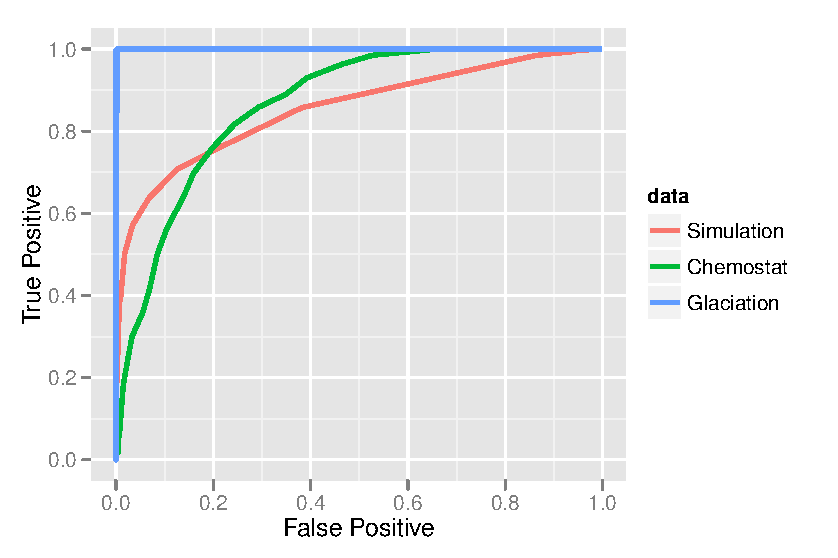
\includegraphics{rocplot} 

\end{kframe}}
\end{knitrout}

\end{figure}

\subsection{ Parameter distributions}

We can also look at the bootstraps of the parameters.  Another helper function will reformat this data from reps list.  The fit column uses a two-letter code to indicate first what model was used to simulate the data, and then what model was fit to the data.  For instance, AB means the data was simulated from model A (the null, OU model) but fit to B. 

\begin{knitrout}
\definecolor{shadecolor}{rgb}{.97, .97, .97}{\color{fgcolor}\begin{kframe}
\begin{flushleft}
\ttfamily\noindent
\hlsymbol{pars}{\ }\hlassignement{\usebox{\hlnormalsizeboxlessthan}-}{\ }\hlfunctioncall{parameter\usebox{\hlnormalsizeboxunderscore}bootstraps}\hlkeyword{(}\hlsymbol{reps}\hlkeyword{)}\hspace*{\fill}\\
\hlstd{}\hlfunctioncall{head}\hlkeyword{(}\hlsymbol{pars}\hlkeyword{)}\mbox{}
\normalfont
\end{flushleft}
\begin{verbatim}
##     value parameter fit rep
## 1   2.440        Ro  AA   1
## 2 604.066     theta  AA   1
## 3 146.492     sigma  AA   1
## 4   1.782        Ro  AB   1
## 5 640.402     theta  AB   1
## 6 140.099     sigma  AB   1
\end{verbatim}
\end{kframe}}
\end{knitrout}


There are lots of options for visualizing this relatively high-dimensional data, which we can easily explore with a few commands from the \texttt{ggplot2} package. For instance, we can look at average and range of parameters estimated in the bootstraps of each model: 

\begin{figure}[H]
\begin{knitrout}
\definecolor{shadecolor}{rgb}{.97, .97, .97}{\color{fgcolor}\begin{kframe}
\begin{flushleft}
\ttfamily\noindent
\hlfunctioncall{require}\hlkeyword{(}\hlsymbol{Hmisc}\hlkeyword{)}\hspace*{\fill}\\
\hlstd{}\hlfunctioncall{ggplot}\hlkeyword{(}\hlfunctioncall{subset}\hlkeyword{(}\hlsymbol{pars}\hlkeyword{,}{\ }\hlsymbol{fit}{\ }\hlkeyword{\usebox{\hlnormalsizeboxpercent}in\usebox{\hlnormalsizeboxpercent}}{\ }\hlfunctioncall{c}\hlkeyword{(}\hlstring{"{}AA"{}}\hlkeyword{,}{\ }\hlstring{"{}BB"{}}\hlkeyword{)}\hlkeyword{)}\hlkeyword{,}{\ }\hlfunctioncall{aes}\hlkeyword{(}\hlsymbol{fit}\hlkeyword{,}{\ }\hlsymbol{value}\hlkeyword{)}\hlkeyword{)}{\ }\hlkeyword{+}\hspace*{\fill}\\
\hlstd{}{\ }{\ }\hlfunctioncall{stat\usebox{\hlnormalsizeboxunderscore}summary}\hlkeyword{(}\hlargument{fun.y}{\ }\hlargument{=}{\ }\hlsymbol{mean}\hlkeyword{,}{\ }\hlargument{geom}{\ }\hlargument{=}{\ }\hlstring{"{}bar"{}}\hlkeyword{,}{\ }\hlargument{position}{\ }\hlargument{=}{\ }\hlstring{"{}dodge"{}}\hlkeyword{)}{\ }\hlkeyword{+}\hspace*{\fill}\\
\hlstd{}{\ }{\ }\hlfunctioncall{stat\usebox{\hlnormalsizeboxunderscore}summary}\hlkeyword{(}\hlargument{fun.data}{\ }\hlargument{=}{\ }\hlsymbol{median\usebox{\hlnormalsizeboxunderscore}hilow}\hlkeyword{,}{\ }\hlargument{geom}{\ }\hlargument{=}{\ }\hlstring{"{}pointrange"{}}\hlkeyword{,}\hspace*{\fill}\\
\hlstd{}{\ }{\ }{\ }{\ }{\ }{\ }{\ }{\ }{\ }{\ }{\ }{\ }{\ }{\ }{\ }\hlargument{position}{\ }\hlargument{=}{\ }\hlfunctioncall{position\usebox{\hlnormalsizeboxunderscore}dodge}\hlkeyword{(}\hlargument{width}{\ }\hlargument{=}{\ }\hlnumber{0.90}\hlkeyword{)}\hlkeyword{,}{\ }\hlargument{conf.int}{\ }\hlargument{=}{\ }\hlnumber{0.95}\hlkeyword{)}{\ }\hlkeyword{+}\hspace*{\fill}\\
\hlstd{}{\ }{\ }\hlfunctioncall{facet\usebox{\hlnormalsizeboxunderscore}wrap}\hlkeyword{(}\hlkeyword{\urltilda{}}\hlsymbol{parameter}\hlkeyword{,}{\ }\hlargument{scales}\hlargument{=}\hlstring{"{}free\usebox{\hlnormalsizeboxunderscore}y"{}}\hlkeyword{)}\mbox{}
\normalfont
\end{flushleft}


\centering{}\includegraphics{parplot} 

\end{kframe}}
\end{knitrout}

\end{figure}


%\subsection{Visualizing the simulation replicates}
%
%The \texttt{reps} list also contains the simulation data from each replicate
%\setkeys{Gin}{width=0.95\textwidth}
%
%\begin{figure}[H]
%<<<repsplot, fig.width=7>>=
%sims <- get_replicates(reps)
%ggplot(sims) + geom_line(aes(time, value, group=rep), alpha=0.1) + facet_wrap(~model)
%@
%\end{figure}
%\setkeys{Gin}{width=0.5\textwidth}

\section{Computing summary statistics with improved sampling}

Autocorrelation performs particularly poorly on the examples in the text, falling on approximately the 1:1 line in the ROC curves.  This example goes through the steps to demonstrate that in a sufficiently-frequently sampled timeseries, autocorrelation does contain *some* signal of early warning, it is simply a weaker signal than the corresponding analysis with variance, which in turn is weaker than the model-based approach. This example also illustrates the use of some of the summary statistics tools.   


We begin by running the individual based simulation, supplied in our helper package, populationdynamics, with~1500 sample points, instead of the 40 shown in the text.   

\begin{knitrout}
\definecolor{shadecolor}{rgb}{.97, .97, .97}{\color{fgcolor}\begin{kframe}
\begin{flushleft}
\ttfamily\noindent
\hlfunctioncall{require}\hlkeyword{(}\hlsymbol{populationdynamics}\hlkeyword{)}\hspace*{\fill}\\
\hlstd{}\hlsymbol{pars}{\ }\hlassignement{=}{\ }\hlfunctioncall{c}\hlkeyword{(}\hlargument{Xo}{\ }\hlargument{=}{\ }\hlnumber{730}\hlkeyword{,}{\ }\hlargument{e}{\ }\hlargument{=}{\ }\hlnumber{0.5}\hlkeyword{,}{\ }\hlargument{a}{\ }\hlargument{=}{\ }\hlnumber{100}\hlkeyword{,}{\ }\hlargument{K}{\ }\hlargument{=}{\ }\hlnumber{1000}\hlkeyword{,}{\ }\hlargument{h}{\ }\hlargument{=}{\ }\hlnumber{200}\hlkeyword{,}{\ }\hlargument{i}{\ }\hlargument{=}{\ }\hlnumber{0}\hlkeyword{,}{\ }\hlargument{Da}{\ }\hlargument{=}{\ }\hlnumber{.09}\hlkeyword{,}{\ }\hlargument{Dt}{\ }\hlargument{=}{\ }\hlnumber{0}\hlkeyword{,}{\ }\hlargument{p}{\ }\hlargument{=}{\ }\hlnumber{2}\hlkeyword{)}\hspace*{\fill}\\
\hlstd{}\hlsymbol{time}\hlassignement{=}\hlfunctioncall{seq}\hlkeyword{(}\hlnumber{0}\hlkeyword{,}{\ }\hlnumber{500}\hlkeyword{,}{\ }\hlargument{length}\hlargument{=}\hlnumber{1500}\hlkeyword{)}\hspace*{\fill}\\
\hlstd{}\hlsymbol{sn}{\ }\hlassignement{\usebox{\hlnormalsizeboxlessthan}-}{\ }\hlfunctioncall{saddle\usebox{\hlnormalsizeboxunderscore}node\usebox{\hlnormalsizeboxunderscore}ibm}\hlkeyword{(}\hlsymbol{pars}\hlkeyword{,}\hlsymbol{time}\hlkeyword{)}\hspace*{\fill}\\
\hlstd{}\hlsymbol{X}{\ }\hlassignement{\usebox{\hlnormalsizeboxlessthan}-}{\ }\hlfunctioncall{data.frame}\hlkeyword{(}\hlargument{time}\hlargument{=}\hlsymbol{time}\hlkeyword{,}{\ }\hlargument{value}\hlargument{=}\hlsymbol{sn}\hlkeyword{\usebox{\hlnormalsizeboxdollar}}\hlsymbol{x1}\hlkeyword{)}\mbox{}
\normalfont
\end{flushleft}
\end{kframe}}
\end{knitrout}


We compute the observed value of Kendall's tau for the autocorrelation computed in a moving window over the data.  (The warningtrend function is just a wrapper for the base function cor.test, which handles different window sizes.  The default uses half the length of the timeseries.)  

\begin{knitrout}
\definecolor{shadecolor}{rgb}{.97, .97, .97}{\color{fgcolor}\begin{kframe}
\begin{flushleft}
\ttfamily\noindent
\hlsymbol{observed}{\ }\hlassignement{\usebox{\hlnormalsizeboxlessthan}-}{\ }\hlfunctioncall{warningtrend}\hlkeyword{(}\hlsymbol{X}\hlkeyword{,}{\ }\hlsymbol{window\usebox{\hlnormalsizeboxunderscore}autocorr}\hlkeyword{)}\hspace*{\fill}\\
\hlstd{}\hlsymbol{observed}\mbox{}
\normalfont
\end{flushleft}
\begin{verbatim}
##    tau 
## 0.8628 
\end{verbatim}
\end{kframe}}
\end{knitrout}


While this gives us single value which is useful for statistical comparisons that follow, recall that it is more common to simply plot the autocorrelation computed in this manner, and the increase is just the visual pattern.  

\begin{figure}[H]
\begin{knitrout}
\definecolor{shadecolor}{rgb}{.97, .97, .97}{\color{fgcolor}\begin{kframe}
\begin{flushleft}
\ttfamily\noindent
\hlsymbol{npts}{\ }\hlassignement{\usebox{\hlnormalsizeboxlessthan}-}{\ }\hlfunctioncall{length}\hlkeyword{(}\hlsymbol{X}\hlkeyword{[[}\hlstring{"{}value"{}}\hlkeyword{]}\hlkeyword{]}\hlkeyword{)}\hspace*{\fill}\\
\hlstd{}\hlsymbol{autocorrelation}{\ }\hlassignement{\usebox{\hlnormalsizeboxlessthan}-}{\ }\hlfunctioncall{window\usebox{\hlnormalsizeboxunderscore}autocorr}\hlkeyword{(}\hlsymbol{X}\hlkeyword{[[}\hlstring{"{}value"{}}\hlkeyword{]}\hlkeyword{]}\hlkeyword{,}{\ }\hlargument{windowsize}\hlargument{=}\hlsymbol{npts}\hlkeyword{/}\hlnumber{2}\hlkeyword{)}\hspace*{\fill}\\
\hlstd{}\hlsymbol{autocorrelation}{\ }\hlassignement{\usebox{\hlnormalsizeboxlessthan}-}{\ }\hlfunctioncall{c}\hlkeyword{(}\hlfunctioncall{rep}\hlkeyword{(}\hlnumber{NA}\hlkeyword{,}{\ }\hlsymbol{npts}\hlkeyword{/}\hlnumber{2}\hlkeyword{-}\hlnumber{1}\hlkeyword{)}\hlkeyword{,}{\ }\hlsymbol{autocorrelation}\hlkeyword{)}\hspace*{\fill}\\
\hlstd{}\hlfunctioncall{plot}\hlkeyword{(}\hlsymbol{X}\hlkeyword{[[}\hlstring{"{}time"{}}\hlkeyword{]}\hlkeyword{]}\hlkeyword{,}{\ }\hlsymbol{autocorrelation}\hlkeyword{,}{\ }\hlargument{type}\hlargument{=}\hlstring{"{}l"{}}\hlkeyword{)}\mbox{}
\normalfont
\end{flushleft}


\centering{}\includegraphics{plot_autocorr} 

\end{kframe}}
\end{knitrout}

\end{figure}

To bootstrap the estimate of tau, we need to be able to simulate under a null and test model.  We use our models of a stable system and a system approaching a collapse to do this.  We first estimate the model parameters from the data, 

\begin{knitrout}
\definecolor{shadecolor}{rgb}{.97, .97, .97}{\color{fgcolor}\begin{kframe}
\begin{flushleft}
\ttfamily\noindent
\hlsymbol{A}{\ }\hlassignement{\usebox{\hlnormalsizeboxlessthan}-}{\ }\hlfunctioncall{stability\usebox{\hlnormalsizeboxunderscore}model}\hlkeyword{(}\hlsymbol{X}\hlkeyword{,}{\ }\hlstring{"{}OU"{}}\hlkeyword{)}\hspace*{\fill}\\
\hlstd{}\hlsymbol{B}{\ }\hlassignement{\usebox{\hlnormalsizeboxlessthan}-}{\ }\hlfunctioncall{stability\usebox{\hlnormalsizeboxunderscore}model}\hlkeyword{(}\hlsymbol{X}\hlkeyword{,}{\ }\hlstring{"{}LSN"{}}\hlkeyword{)}\mbox{}
\normalfont
\end{flushleft}
\end{kframe}}
\end{knitrout}


and then we can simulate some replicates

\begin{knitrout}
\definecolor{shadecolor}{rgb}{.97, .97, .97}{\color{fgcolor}\begin{kframe}
\begin{flushleft}
\ttfamily\noindent
\hlsymbol{nreps}{\ }\hlassignement{\usebox{\hlnormalsizeboxlessthan}-}{\ }\hlnumber{500}\hspace*{\fill}\\
\hlstd{}\hlsymbol{Asim}{\ }\hlassignement{\usebox{\hlnormalsizeboxlessthan}-}{\ }\hlfunctioncall{simulate}\hlkeyword{(}\hlsymbol{A}\hlkeyword{,}{\ }\hlsymbol{nreps}\hlkeyword{)}\hspace*{\fill}\\
\hlstd{}\hlsymbol{Bsim}{\ }\hlassignement{\usebox{\hlnormalsizeboxlessthan}-}{\ }\hlfunctioncall{simulate}\hlkeyword{(}\hlsymbol{B}\hlkeyword{,}{\ }\hlsymbol{nreps}\hlkeyword{)}\mbox{}
\normalfont
\end{flushleft}
\end{kframe}}
\end{knitrout}



We tidy up the data a bit; columns should be variables, not replicates.   
\begin{knitrout}
\definecolor{shadecolor}{rgb}{.97, .97, .97}{\color{fgcolor}\begin{kframe}
\begin{flushleft}
\ttfamily\noindent
\hlfunctioncall{require}\hlkeyword{(}\hlsymbol{reshape2}\hlkeyword{)}\hspace*{\fill}\\
\hlstd{}\hlsymbol{Asim}{\ }\hlassignement{\usebox{\hlnormalsizeboxlessthan}-}{\ }\hlfunctioncall{melt}\hlkeyword{(}\hlsymbol{Asim}\hlkeyword{,}{\ }\hlargument{id}\hlargument{=}\hlstring{"{}time"{}}\hlkeyword{)}\hspace*{\fill}\\
\hlstd{}\hlsymbol{Bsim}{\ }\hlassignement{\usebox{\hlnormalsizeboxlessthan}-}{\ }\hlfunctioncall{melt}\hlkeyword{(}\hlsymbol{Bsim}\hlkeyword{,}{\ }\hlargument{id}\hlargument{=}\hlstring{"{}time"{}}\hlkeyword{)}\hspace*{\fill}\\
\hlstd{}\hlfunctioncall{names}\hlkeyword{(}\hlsymbol{Asim}\hlkeyword{)}\hlkeyword{[}\hlnumber{2}\hlkeyword{]}{\ }\hlassignement{\usebox{\hlnormalsizeboxlessthan}-}{\ }\hlstring{"{}reps"{}}\hspace*{\fill}\\
\hlstd{}\hlfunctioncall{names}\hlkeyword{(}\hlsymbol{Bsim}\hlkeyword{)}\hlkeyword{[}\hlnumber{2}\hlkeyword{]}{\ }\hlassignement{\usebox{\hlnormalsizeboxlessthan}-}{\ }\hlstring{"{}reps"{}}\mbox{}
\normalfont
\end{flushleft}
\end{kframe}}
\end{knitrout}


Now that we have replicates from each process, we can apply the windowed autocorrelation function to each replicate
\begin{knitrout}
\definecolor{shadecolor}{rgb}{.97, .97, .97}{\color{fgcolor}\begin{kframe}
\begin{flushleft}
\ttfamily\noindent
\hlfunctioncall{require}\hlkeyword{(}\hlsymbol{plyr}\hlkeyword{)}\hspace*{\fill}\\
\hlstd{}\hlfunctioncall{require}\hlkeyword{(}\hlsymbol{doMC}\hlkeyword{)}\hspace*{\fill}\\
\hlstd{}\hlfunctioncall{registerDoMC}\hlkeyword{(}\hlkeyword{)}\hspace*{\fill}\\
\hlstd{}\hlsymbol{wsA}{\ }\hlassignement{\usebox{\hlnormalsizeboxlessthan}-}{\ }\hlfunctioncall{ddply}\hlkeyword{(}\hlsymbol{Asim}\hlkeyword{,}{\ }\hlstring{"{}reps"{}}\hlkeyword{,}{\ }\hlsymbol{warningtrend}\hlkeyword{,}{\ }\hlsymbol{window\usebox{\hlnormalsizeboxunderscore}autocorr}\hlkeyword{,}{\ }\hlargument{.parallel}\hlargument{=}\hlnumber{TRUE}\hlkeyword{)}\hspace*{\fill}\\
\hlstd{}\hlsymbol{wsB}{\ }\hlassignement{\usebox{\hlnormalsizeboxlessthan}-}{\ }\hlfunctioncall{ddply}\hlkeyword{(}\hlsymbol{Bsim}\hlkeyword{,}{\ }\hlstring{"{}reps"{}}\hlkeyword{,}{\ }\hlsymbol{warningtrend}\hlkeyword{,}{\ }\hlsymbol{window\usebox{\hlnormalsizeboxunderscore}autocorr}\hlkeyword{,}{\ }\hlargument{.parallel}\hlargument{=}\hlnumber{TRUE}\hlkeyword{)}\mbox{}
\normalfont
\end{flushleft}
\end{kframe}}
\end{knitrout}


And gather and plot the distributions,
\begin{figure}[H]
\begin{knitrout}
\definecolor{shadecolor}{rgb}{.97, .97, .97}{\color{fgcolor}\begin{kframe}
\begin{flushleft}
\ttfamily\noindent
\hlsymbol{tidy}{\ }\hlassignement{\usebox{\hlnormalsizeboxlessthan}-}{\ }\hlfunctioncall{melt}\hlkeyword{(}\hlfunctioncall{data.frame}\hlkeyword{(}\hlargument{null}\hlargument{=}\hlsymbol{wsA}\hlkeyword{\usebox{\hlnormalsizeboxdollar}}\hlsymbol{tau}\hlkeyword{,}{\ }\hlargument{test}\hlargument{=}\hlsymbol{wsB}\hlkeyword{\usebox{\hlnormalsizeboxdollar}}\hlsymbol{tau}\hlkeyword{)}\hlkeyword{)}\hspace*{\fill}\\
\hlstd{}\hlfunctioncall{names}\hlkeyword{(}\hlsymbol{tidy}\hlkeyword{)}{\ }\hlassignement{\usebox{\hlnormalsizeboxlessthan}-}{\ }\hlfunctioncall{c}\hlkeyword{(}\hlstring{"{}simulation"{}}\hlkeyword{,}{\ }\hlstring{"{}value"{}}\hlkeyword{)}\hspace*{\fill}\\
\hlstd{}\hlfunctioncall{beanplot}\hlkeyword{(}\hlsymbol{value}{\ }\hlkeyword{\urltilda{}}{\ }\hlsymbol{simulation}\hlkeyword{,}{\ }\hlsymbol{tidy}\hlkeyword{,}{\ }\hlargument{what}\hlargument{=}\hlfunctioncall{c}\hlkeyword{(}\hlnumber{0}\hlkeyword{,}\hlnumber{1}\hlkeyword{,}\hlnumber{0}\hlkeyword{,}\hlnumber{0}\hlkeyword{)}\hlkeyword{)}\hspace*{\fill}\\
\hlstd{}\hlfunctioncall{abline}\hlkeyword{(}\hlargument{h}\hlargument{=}\hlsymbol{observed}\hlkeyword{,}{\ }\hlargument{lty}\hlargument{=}\hlnumber{2}\hlkeyword{)}\mbox{}
\normalfont
\end{flushleft}


\centering{}\includegraphics{tidybean} 

\end{kframe}}
\end{knitrout}

\end{figure}

and corrsponding ROC plot,
\begin{figure}[H]
\begin{knitrout}
\definecolor{shadecolor}{rgb}{.97, .97, .97}{\color{fgcolor}\begin{kframe}
\begin{flushleft}
\ttfamily\noindent
\hlsymbol{roc}{\ }\hlassignement{\usebox{\hlnormalsizeboxlessthan}-}{\ }\hlfunctioncall{roc\usebox{\hlnormalsizeboxunderscore}data}\hlkeyword{(}\hlsymbol{tidy}\hlkeyword{)}\hspace*{\fill}\\
\hlstd{}\hlfunctioncall{ggplot}\hlkeyword{(}\hlsymbol{roc}\hlkeyword{)}{\ }\hlkeyword{+}{\ }\hlfunctioncall{geom\usebox{\hlnormalsizeboxunderscore}line}\hlkeyword{(}\hlfunctioncall{aes}\hlkeyword{(}\hlsymbol{False.positives}\hlkeyword{,}{\ }\hlsymbol{True.positives}\hlkeyword{)}\hlkeyword{,}{\ }\hlargument{lwd}\hlargument{=}\hlnumber{1}\hlkeyword{)}\mbox{}
\normalfont
\end{flushleft}


\centering{}\includegraphics{anotherroc} 

\end{kframe}}
\end{knitrout}

\end{figure}



Lastly we save the data from each of these examples for future reference.   
\begin{knitrout}
\definecolor{shadecolor}{rgb}{.97, .97, .97}{\color{fgcolor}\begin{kframe}
\begin{flushleft}
\ttfamily\noindent
\hlfunctioncall{save}\hlkeyword{(}\hlargument{list}\hlargument{=}\hlfunctioncall{ls}\hlkeyword{(}\hlkeyword{)}\hlkeyword{,}{\ }\hlargument{file}\hlargument{=}\hlstring{"{}tutorial.rda"{}}\hlkeyword{)}\mbox{}
\normalfont
\end{flushleft}
\end{kframe}}
\end{knitrout}



%\section{Package Installation}




\section*{ }%bibliography
\bibliographystyle{elsarticle-harv}
%\bibliography{/home/cboettig/Documents/Mendeley/bib/library}
%\bibliography{../boettiger}

\end{document}

